\section*{Sequential matrix multiplication}


\subsection*{1) Running Times}
In this section we will check running times of the algorithm running on different sized matrices

\begin{figure}[h!] 
 \center 
 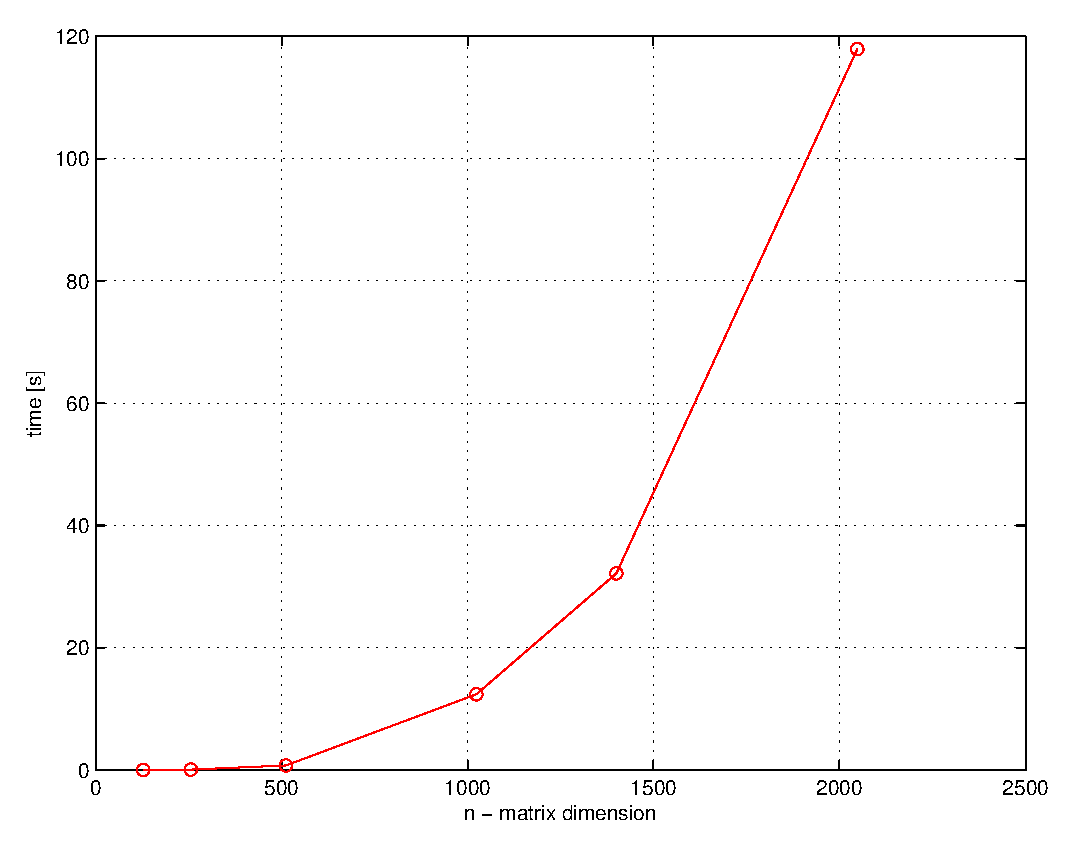
\includegraphics[scale=\figurescale]{./figures/plot21.eps}
 \caption{  \label{fig:} Plot of different running times for sequential matrix multiplication}
 \end{figure}

\begin{figure}[h!] 
 \center 
 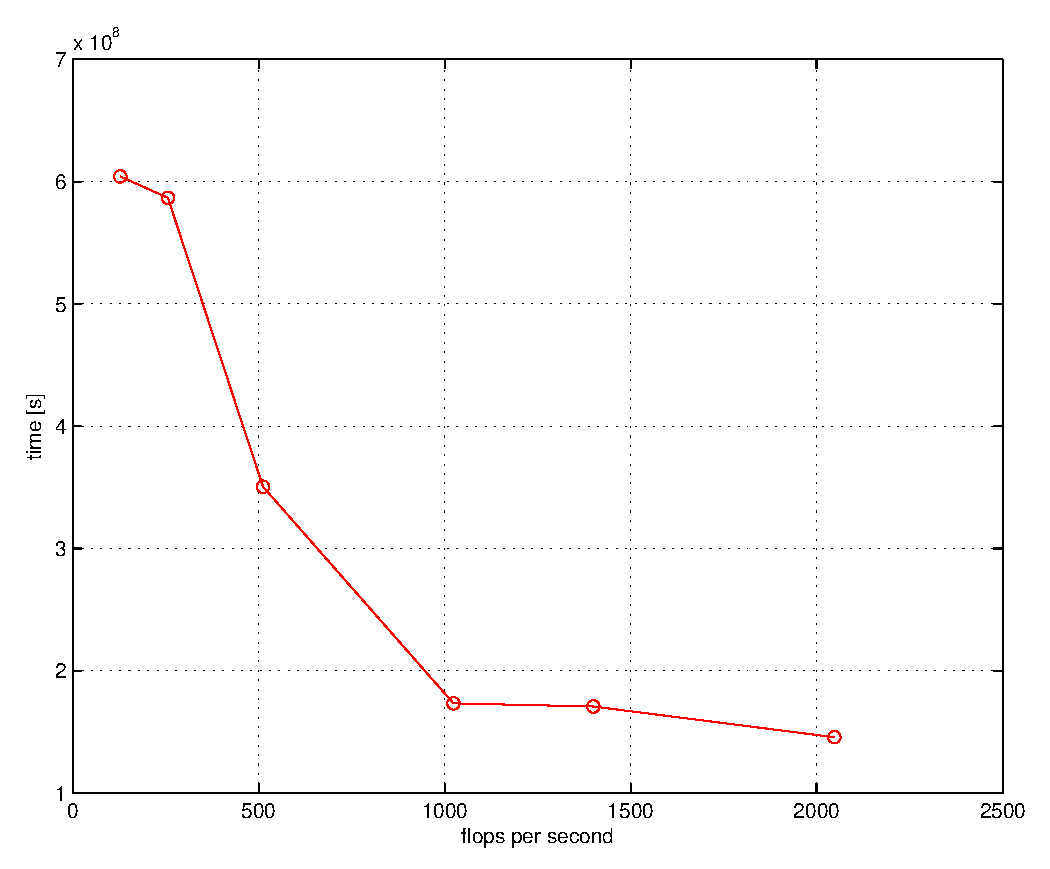
\includegraphics[scale=\figurescale]{./figures/plot22.eps}
 \caption{  \label{fig:flops} Plot of flops per second for the different matrix dimensions}
 \end{figure}

As we can see in Fig. \ref{fig:flops} The rate of flops per second is not constant for different running times. This can be due to the the fact that for the higher dimension matrix multiplication, the amount of data is so big that it has the cache is filled up and most of the time is used for accessing memory instead of doing the actual computing. 



\subsection*{2) Different nested loops}


\begin{figure}[h!] 
 \center 
 \subfloat[]{ 
 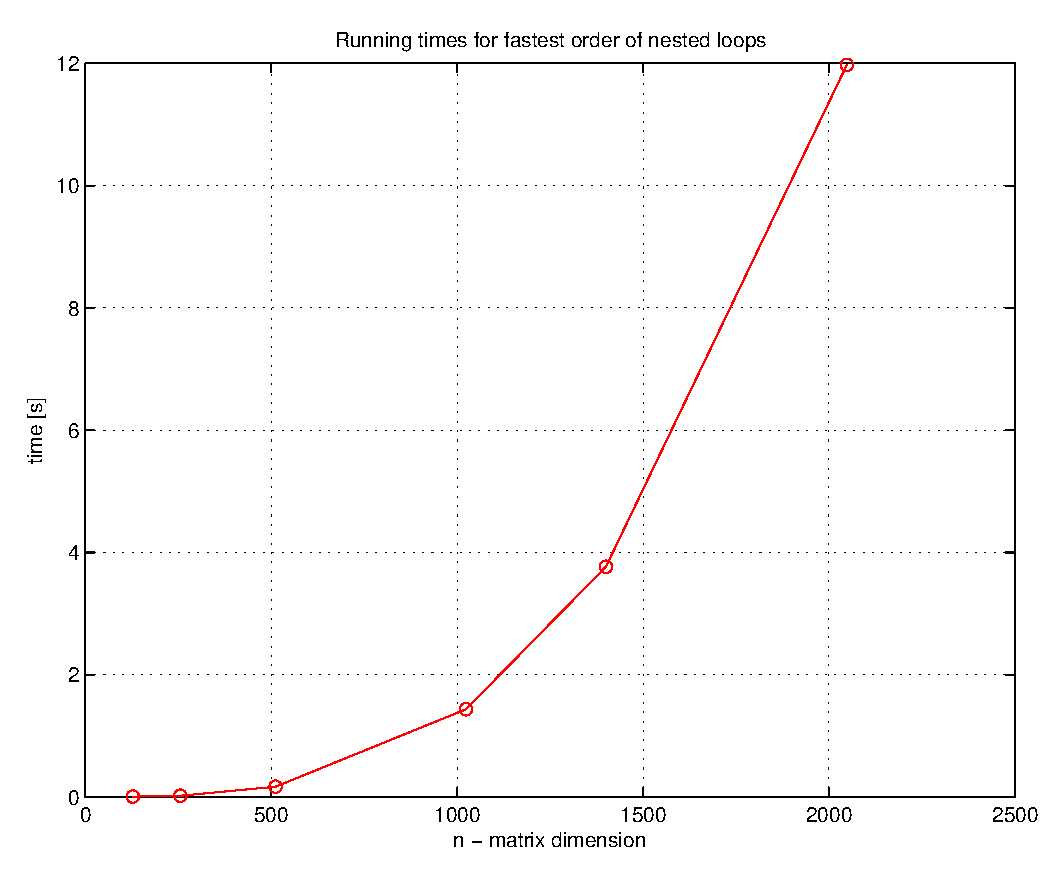
\includegraphics[scale=\figurescale]{./figures/plot23.eps} }
 \subfloat[]{ 
 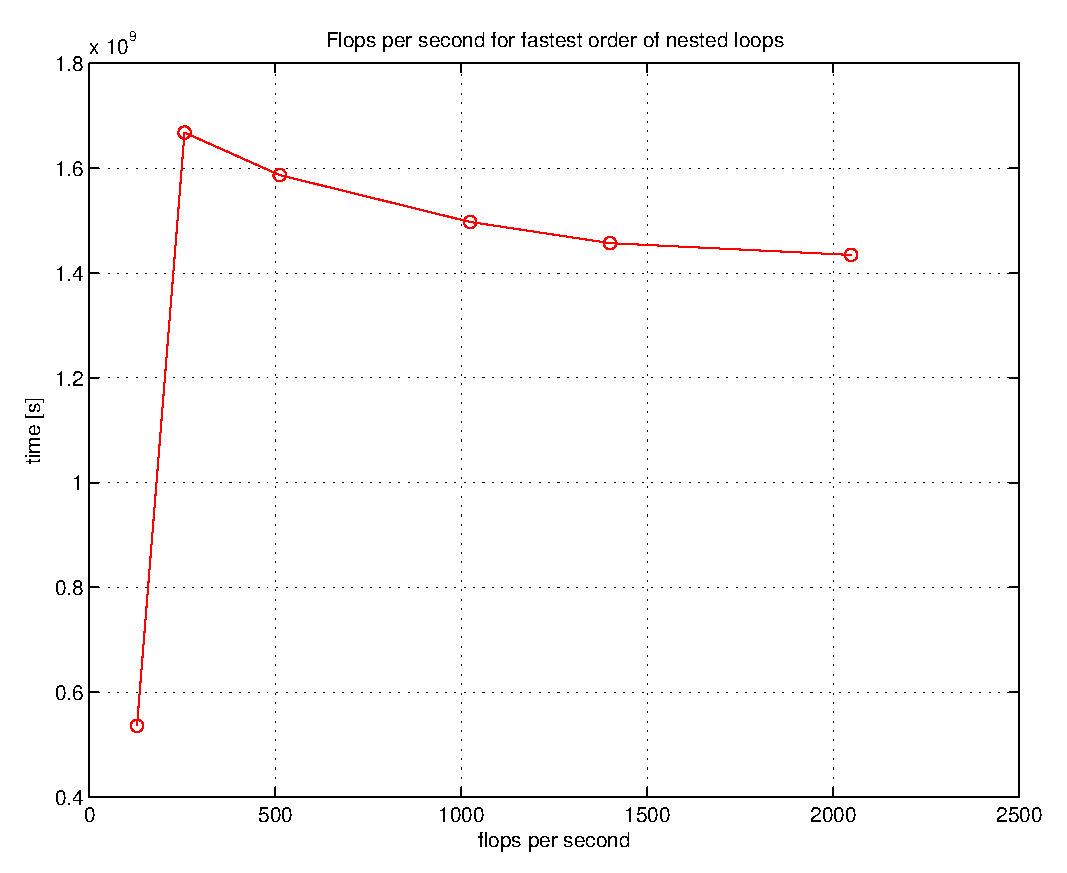
\includegraphics[scale=\figurescale]{./figures/plot24.eps} }
 \caption{ Running times and flops/s for fastest order of nested loops \label{fig:fastest}}
 \end{figure}

\begin{figure}[h!] 
 \center 
 \subfloat[]{ 
 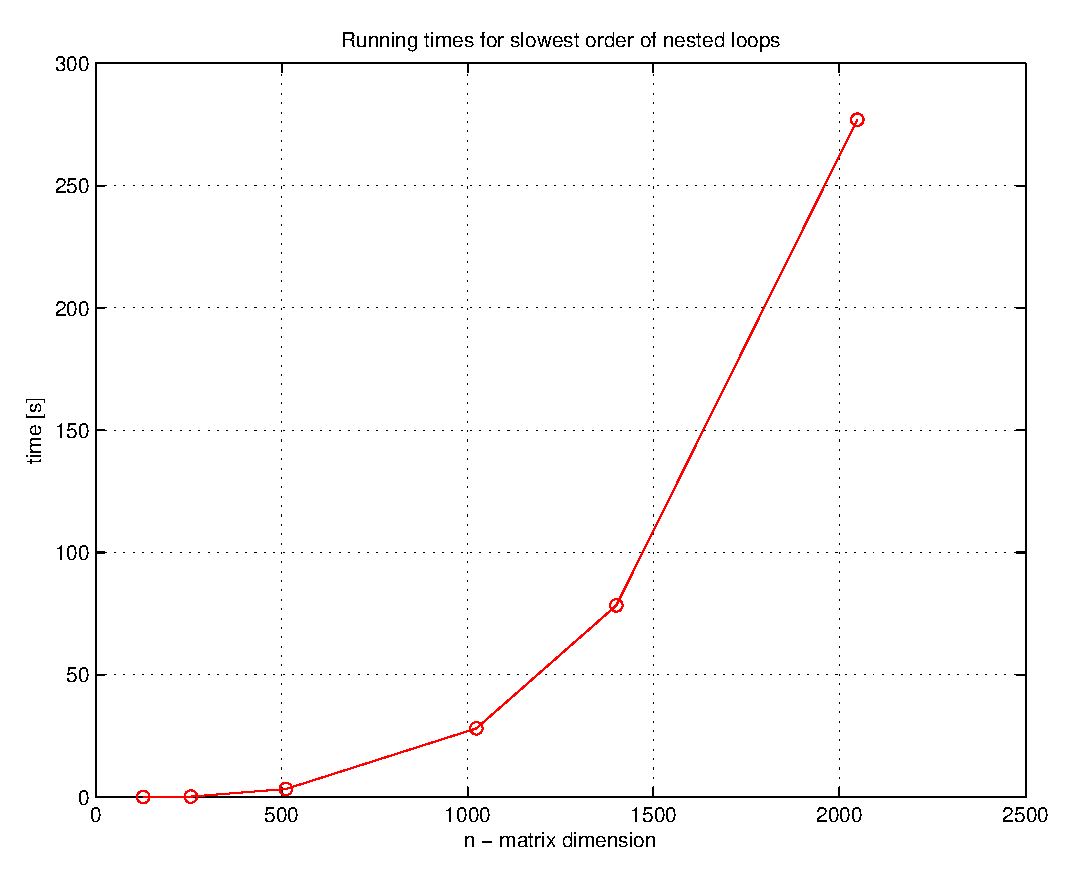
\includegraphics[scale=\figurescale]{./figures/plot25.eps} }
 \subfloat[]{ 
 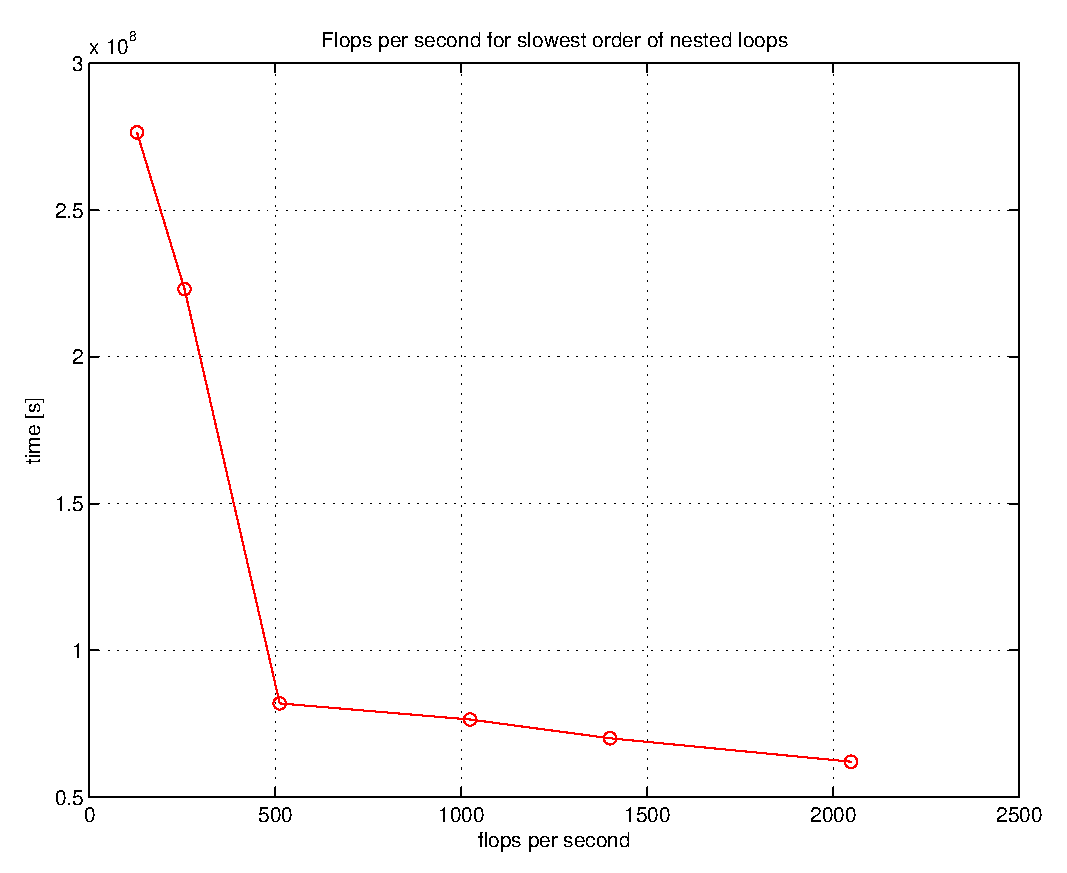
\includegraphics[scale=\figurescale]{./figures/plot26.eps} }
 \caption{ Running times and flops/s for slowest order of nested loops \label{fig:slowest}}
 \end{figure}


Testing different orders of i j k for the nested loops, it was obvious that the order $j k i$ was the fastest and the order $ i k j$ where the slowest.  The different running times and flops/s can be seen in Fig. \ref{fig:fastest} and Fig. \ref{fig:slowest}. The reason for the big difference in performance is mainly due to how the data is accessed in memory. For a certain order of the iterations, the property of prefetching using spacial locality is being taken advantage of. This means that when the memory is loaded into the cache for the first element of a matrix a big chunk is also loaded into memory, following the first element in the address space. For a certain order of iteration, the elements that is prefetched is used first, leading to fewer cache misses and a faster performance.



